\documentclass[11pt,a4paper]{article}

\usepackage{fullpage}
\usepackage{hyperref}
\usepackage{graphicx}
\usepackage{amsmath}
\usepackage{subcaption}
\usepackage{booktabs}
\usepackage{listings}
\graphicspath{ {Data/} }
\usepackage{fancyhdr}
\pagestyle{fancy}
\fancyhf{}

\renewcommand{\headrulewidth}{0pt}
\renewcommand{\footrulewidth}{0pt}

\fancypagestyle{firstpagefooter} {
	\lfoot{\tiny{Version: 21.09.2017}}
	\cfoot{}
	\rfoot{\thepage}
	
}

\lfoot{Name: Simon Bodvarsson Legi: 16-931-685}
\rfoot{\thepage}

\begin{document}

\title{Advanced Systems Lab Report\\ \normalsize{Autumn Semester 2017}}
\author{Name: Simon Bodvarsson\\Legi: 16-931-685}
\date{
	\vspace{4cm}
	\textbf{Grading} \\
	\vspace{0.5cm}
	\begin{tabular}{|c|c|}
		\hline  \textbf{Section} & \textbf{Points} \\
		\hline  1                &                 \\ 
		\hline  2                &                 \\ 
		\hline  3                &                 \\ 
		\hline  4                &                 \\ 
		\hline  5                &                 \\ 
		\hline  6                &                 \\ 
		\hline  7                &                 \\ 
		\hline \hline Total      &                 \\
		\hline 
	\end{tabular} 
}
\maketitle
\thispagestyle{firstpagefooter}

\newpage

\section{System Overview (75 pts)}

\begin{figure}
\centering
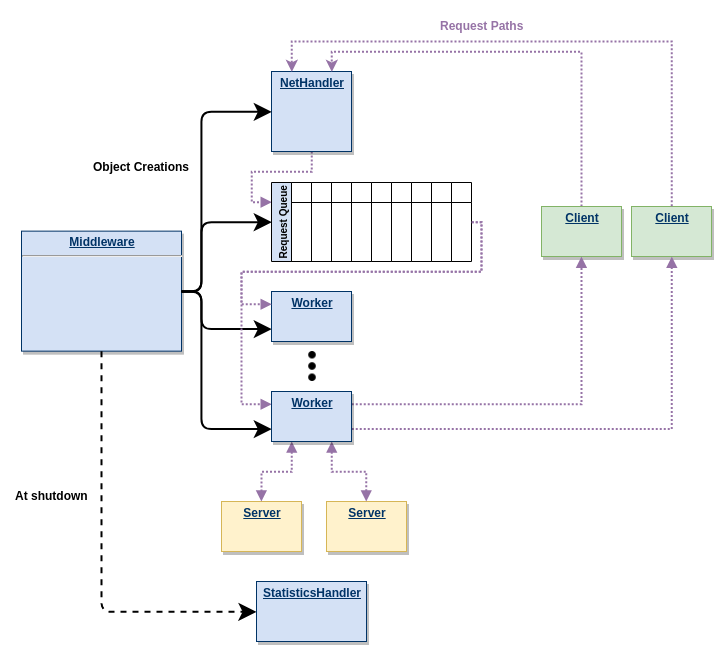
\includegraphics[width=1\textwidth]{system_diagram}
\caption{A view of the middleware system and its components. The blue rectangles represent the Java objects which are parts of the middleware. The black arrows represent object creations. The green and beige rectangles represent the client VMs and server VMs, respectively. The purple arrows show the path a request takes through the system. A request is initially sent by the client to the middleware, where it is handled by the NetHandler. It is then added to the request queue where it waits for an available worker. A worker removes the request from the queue, forwards it to one or more servers and awaits the server response before finally responding to the client according to the server response. At shut down the middleware creates a StatisticsHandler which gathers statistics from all Workers, aggragates them and writes them to files.}
\label{fig:system_diagram}
\end{figure}

The system was implemented as shown in figure \ref{fig:system_diagram}. At system start up, the \texttt{MyMiddleware} object creates a \texttt{LinkedBlockingQueue} for requests, a \texttt{NetHandler} object which takes care of accepting new incoming connections from clients and adding new requests made by the clients to the RequestQueue. According to the command line arguments given by the user, the middleware will create \texttt{Worker} objects which remove requests from the queue, forward them to the servers and answer the client which made the request. The \texttt{NetHandler}, \texttt{StatisticsHandler} and \texttt{Worker} objects are each assigned to its own thread.\\

\subsection{NetHandler Class}
The \texttt{NetHandler} class uses Java's NIO API for handling connections to clients. Java NIO allows for simple non-blocking IO. The \texttt{NetHandler} object contains a \texttt{Selector} which will repeatedly check for new available client connections to open and check if any existing client connections are ready to be read. This check is blocking and allows us to avoid using a hot loop to check for new requests.\\
Whenever a client connection is read, the \texttt{NetHandler} object parses the message to check if it contains a complete request. In the case where a complete request is contained within the message, the \texttt{NetHandler} creates a new \texttt{Request} object and pushes it onto the request queue. If an incomplete request is found, the buffer of is rewound to make the unused bytes readable again.

\subsection{Request Class}
We implement an abstract class, \texttt{Request}, and two subclasses: \texttt{GetRequest} and \texttt{SetRequest} which are used to contain the full message string and relevant request information such as: keys, number of keys, timestamp when request was added to the request queue and the socket channel used for client communication.


\subsection{Linked Blocking Queue}
A linked blocking queue was chosen as the implementation for the RequestsQueue. Whenever a worker tries to retrieve a request from the queue, the worker's thread is blocked until a request is available. This approach allows us to retrieve elements without repeatedly checking, wasting CPU cycles. Moreover, the linked blocking queue is thread safe, ensuring that no two workers retrieve the same request. 

\subsection{Worker Class}
The \texttt{Workers} handle communication with the servers and responses to the clients. They also perform logging of various statistics related to the experiments. Each \texttt{Worker} is assigned its own thread.

At creation, each worker will connect to all the servers before trying to retrieve a \texttt{Requests} from the request queue. The queue will block the worker thread until a request is available. When a request is available, the \texttt{worker} retrieves it from the queue, updates the relevant statistics according to the information in the request (request type, request length, queue waiting time and queue length), parses the request if needed, forwards the request to the servers, measures the service time and finally forwards the answer from the server to the client.

Rather than use Java's NIO to handle the communication with the servers like the \texttt{NetHandler}, the simpler Java IO API was used. This approach causes reading the response from the server to be blocking. This was deemed to not be a hindrance since the worker-thread would not have any relevant work to do while waiting for the response, unlike the \texttt{NetHandler} which will use this time to either handle other clients or to accept new connections. 

\begin{figure}
\centering
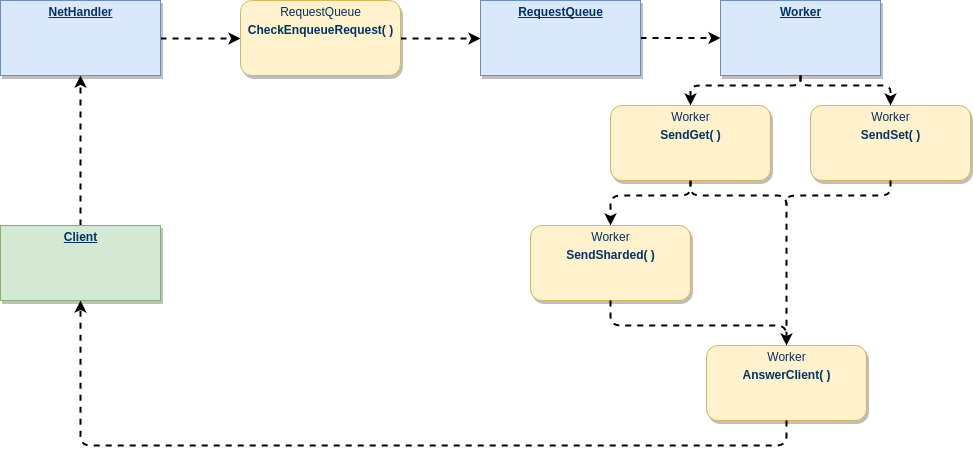
\includegraphics[width=1\textwidth]{request_paths}
\caption{A view of the paths a request takes through the middleware. The black arrows represent the paths a request takes. The blue rectangles represent the Java objects which are parts of the middleware. The beige rectangles represent function calls of those objects. In the case of branching paths, the type of request and whether \texttt{sharded=true} determines which path is chosen. The servers are not shown on this diagram for the sake of clarity. Server communication takes place within the \texttt{SendGet}, \texttt{SendSet} and \texttt{SendSharded} functions of the worker class.}
\label{fig:request_paths}
\end{figure}

\subsubsection{Handling SET-requests}
When handling SET requests, the request needs to be sent to all servers. The request does not need to be processed or changed before forwarding it to the server. Using Java IO sockets we simply write the request to the output stream to each server and flush it. We read the responses from the servers in the same order they were sent. We read from the input stream of the socket, checking for every response if any server responds with the error message "NOT\_STORED\textbackslash r\textbackslash
n". If no server responds with the error message, the message "STORED\textbackslash r\textbackslash n" is sent to the client. If any client responds with the error message, we send the error message "NOT\_STORED\textbackslash r\textbackslash n" to the client using the socket channel contained in the Request object.

\subsubsection{Handling GET-requests}
When handling GET requests, the worker will choose a server to use in a round robin fashion, choosing server $i+1 \mod n_{servers}$ if server $i$ was used for the last GET request. Similar to how SET requests are handled, we simply write the request from the client to the output stream to the server and flush it. We then read lines until a line starting with "END\textbackslash r\textbackslash n" is read indicating that the full response has been read. If the full response is only comprised of "END" we consider the request to have missed, incrementing the count of cache misses encountered in the worker. The response consisting of all the lines read from the server is then sent to the client using the socket channel contained in the Request object.

\subsubsection{Handling Sharded MultiGet-Requests}
If sharded GET requests are enabled and a GET request with multiple keys is retrieved from the queue, we split the keys to be retrieved from different servers. We create $n$ shards where $n = \min (n_{servers}, n_{keys})$. For each shard we create a new GET request with $l = n_{keys}/n$ keys by appending $l$ of the original keys to the string "get". Any keys that are remaining from the integer division ($l = n_{keys}/n$) are added to the last shard. We assign one server to each shard in the same round robin approach as in the normal GET request case. Each shard is then sent to its assigned server using the output stream of its socket. We gather the server responses in the same order as the shards were sent in. For each server, we read all lines sent from the server and remove the string "END\textbackslash r \textbackslash n" from the end. We then append all lines from all servers before finally adding the string "END\textbackslash r \textbackslash n" to the end of the combined response. This combined response is then sent to the client in the same way as for other request types.

\subsubsection{Statistics}
All statistics are measured on a per worker basis for time windows of 4 seconds. The statistics of all workers are aggregated at system shut down. Before handling every request, the \texttt{worker} will check if 4 seconds have passed since the last time statistics of the worker were aggregated. If 4 seconds have passed, all the gathered statistics since the last aggregate are added to lists which contain the statistics for previous time windows and the statistics variables are then reset. In this way the worker thread gathers statistics for every 4 second window. All of the statistics in the worker are stored in memory and are not written to file until the middleware is shut down (See subsection: 1.5 System Shut Down).\\

The statistics gathered are: Count of each request type, number of cache misses, length of request queue, average waiting time in queue, server service time for each request type, throughput, average number of keys in multi-gets.

\subsubsection{Server Service Time}
When a worker thread has sent a complete request to all the necessary servers it will start measuring the service time of the server using System.nanoTime(). When the full response has been read from the servers, the measurement is stopped. This approach is useful to estimate the service time of each request type but also includes the latency between middleware and server as well as the parsing time of the responses for the worker. 

An attempt was made to subtract the network effects by doing a ping measurement from middleware to server before the start of the experiments. The ping measurement turned out to have much too high variation to be of any use in this case and was not used.

\subsubsection{Response Time}
The response time measurements for requests are initiated when the request is put into the request queue and the time stamp is added as a field variable of the request object. When a worker thread has successfully sent the response to the client, the response time measurement is stopped and added to the worker's list of measurements.

\subsection{System Shut Down}
When the middleware is shut down (e.g. with a \texttt{CTRL+C} command) the middleware creates a \texttt{StatisticsHandler} object which accesses the gathered statistics of all \texttt{Workers} and aggregates them, prints them to the standard output and finally logs them to files in a timestamped folder. The \texttt{StatisticsHandler} outputs 4 files. These are MeasurementTable.csv, ResponseTimeHistogram.csv, statistics.csv and error.log.\\ MeasurementTable.csv contains for each timewindow: counts of each request type, average throughput of workers, average queue length, average waiting time in queue for requests and average service times for each request type. \\ ResponseTimeHistogram.csv contains a histogram of the response times of the requests consisting of upper time limits in 100s of $\mu$s for each bucket and the number of requests in each bucket. \\ Statistics.csv contains info on the set up of the middleware: Number of worker threads, number of servers, if reads are sharded or not and the cache miss ratio for the experiment. \\ error.log will contain any error messages that were encountered in the middleware at run time.


\newpage
\section{Baseline without Middleware (75 pts)}

In this experiments we study the performance characteristics of the memtier clients and memcached servers. First we experiment with one server and three client machines and later we experiment with two servers and a single client machine.

\subsection{One Server}

For an experiment set-up with 1 server and 3 client machines with a single instance of Memtier Benchmark each and 2 threads per Memtier instance, we measure the throughput and response time for various values of virtual clients per thread.

The experiments are performed for both a read-only (GET) and a write-only (SET) workload and for the following values of virtual clients per thread: VC$=\{ 1, 4, 8, 16, 24, 32, 40\}$. Each experiment is repeated 3 times. We calculate the total number of clients as $N\_clients = CM \cdot NM \cdot CT \cdot VC$ where $CM$ is the number of client machines, $NM$ is the number of memtier instances per client machine, $CT$ is the number of threads per client instance and $VC$ is the number of virtual clients per memtier instance. In this experiment: $CM=3$, $NM=1$, $CT=2$. The client numbers are therefore $N\_clients = 6\cdot VC = \{6, 24, 48, 96, 144, 192, 240 \}$.

\begin{figure}[h]
\centering
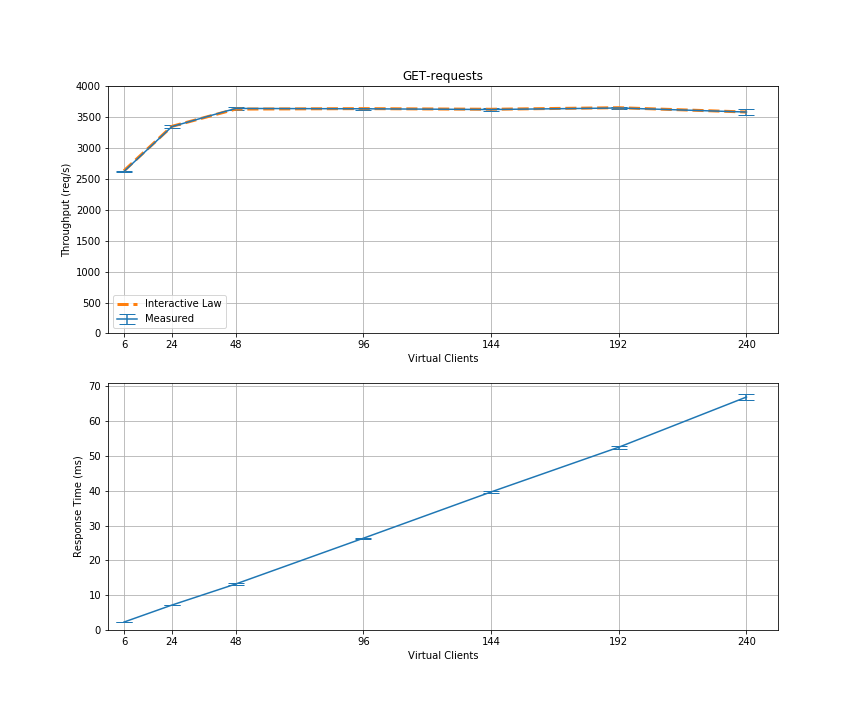
\includegraphics[width=0.9\textwidth]{21/21_get_requests}
\caption{Experiment 2.1: Throughput and response time for a read-only workload. In the upper graph the throughput according to the interactive law has been plotted in addition to the measured throughput. The measurements can be clearly seen to follow the interactive law.}
\label{fig:21get}
\end{figure}

\begin{figure}[h]
\centering
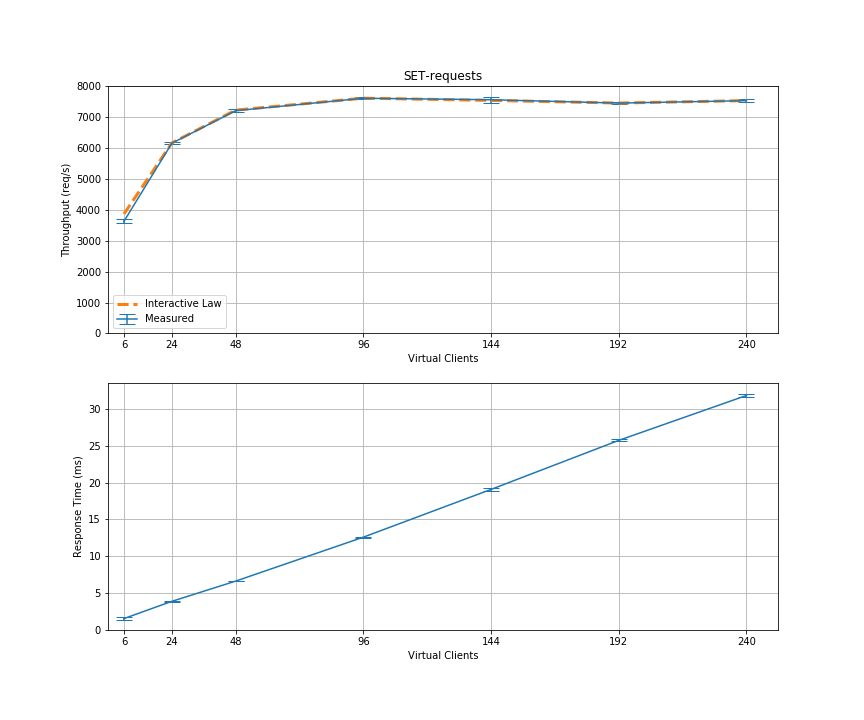
\includegraphics[width=0.9\textwidth]{21/21_set_requests}
\caption{Experiment 2.1: Throughput and response time for a write-only workload. In the upper graph the throughput according to the interactive law has been plotted in addition to the measured throughput. The measurements can be clearly seen to follow the interactive law.}
\label{fig:21set}
\end{figure}

Looking at figures \ref{fig:21get} and \ref{fig:21set} we first note that the measurements clearly follow the interactive law. We also observe that the servers are under-saturated for less than 48 clients, in saturation between 48 and 192 clients and enter the over-saturated phase when client numbers grow above 192. Finally, we note that the maximum throughput achieved is 3650 req/s for the GET requests and 7616 req/s for the SET requests. This represents the maximum throughput a single server can handle. The difference in throughput between these types of requests can likely be attributed to the overhead on the server due to look up in the event of a GET request. We can now estimate the service time of the server for each request type, for GET requests, the server should have a service time of approximately $\frac{1}{3650} = 0.274 ms$ per GET request and $\frac{1}{7616 } = 0.131 ms$ per SET request. 


\subsection{Two Servers}

To test the limits of the client we set up an experiment with two server VMs, one client VM with two instances of memtier with one thread each ($CT=1$) and vary the number of virtual clients (VC) as before. For this experiment we also run write-only and read-only experiments with three repetitions.

\begin{figure}[h]
\centering
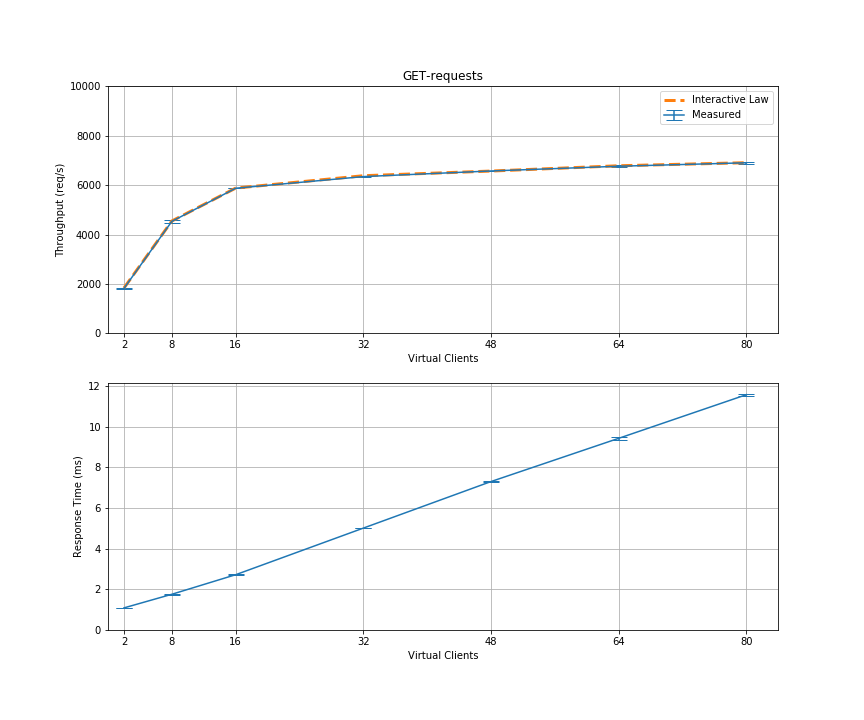
\includegraphics[width=0.9\textwidth]{22/22_get_requests}
\caption{Experiment 2.2: Throughput and response time for a read-only workload on the two server set up. In the upper graph the throughput according to the interactive law has been plotted in addition to the measured throughput. The measurements can be clearly seen to follow the interactive law.}
\label{fig:22get}
\end{figure}

\begin{figure}[h]
\centering
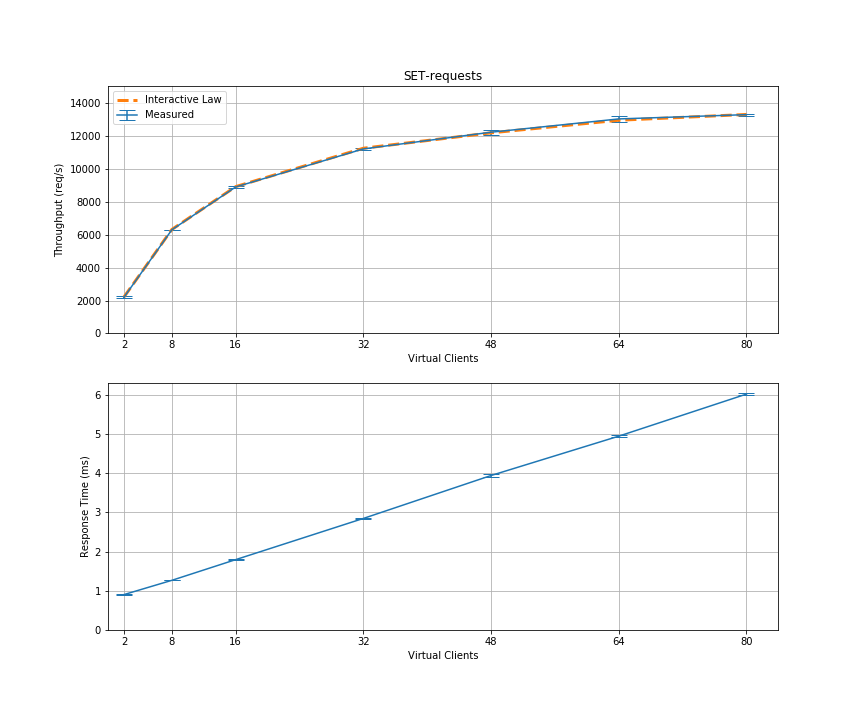
\includegraphics[width=0.9\textwidth]{22/22_set_requests}
\caption{Experiment 2.2: Throughput and response time for a write-only workload on the two server set up. In the upper graph the throughput according to the interactive law has been plotted in addition to the measured throughput. The measurements can be clearly seen to follow the interactive law.}
\label{fig:22set}
\end{figure}

From figures \ref{fig:22get} and \ref{fig:22set} we see that the system remains under saturated for up to about 32 clients in the case of a read-only workload and 64 clients in the case of a write-only workload. The maximum number of clients tested was not sufficient to put the system into an oversaturated phase.

The maximum throughput measured is 6909 req/s for the read-only workload and 13286 req/s for the write-only workload. Comparing these values to the maximum throughput from the single server set-up (GET: 3650 req/s, SET: 7616 req/s), we see that the two server set-up has more than 89\% and 74\% higher maximum throughput for GET requests and SET requests, respectively.
\newpage


\subsection{Conclusion}

\begin{center}
	{Maximum throughput of different VMs.}
	\begin{tabular}{|l|p{2cm}|p{2cm}|p{4cm}|}
		\hline                        & Read-only workload & Write-only workload & Configuration gives max. throughput \\ 
		\hline One memcached server   &          3650      &       7616         &    $VC = 16$                           \\ 
		\hline One load generating VM &          6908      &       13286       &    $VC = 40$                           \\ 
		\hline 
	\end{tabular}
\end{center}

For the read-only workload, we see a 89\% increase in throughput with the two server set-up, while the write-only workload throughput increased by 74\%. This indicates that in our two server set-up, the client must be the bottleneck and in the one server set-up, the server must be the bottleneck.

If the clients were the bottleneck in the single server set-up, then we should see no increase in throughput in the second experiment since it has fewer client VMs but more servers. Since throughput is increased in the second experiment, the server must be the bottleneck in the first experiment.

If the servers were the bottleneck in the two server set-up, then we should see an increase in throughput of around 100\% from the first experiment to the second, since the server was the bottleneck in the first experiment and the servers operate independant of each other. Since the observed increase is lower than 100\%, this indicates that the client is now the bottleneck and cannot keep up with the maximum throughput possible by the servers. Therefore, the client is the bottleneck in the second experiment.

We can therefore conclude that one client VM is more than enough to generate load for one server VM and that the suggested set-up of 3 clients and 3 servers has more than enough clients to test the system. Therefore, we need not worry that the clients will be a bottleneck in the following experiments if they are at least as many as the servers, and that the measured limits of the system will not be due to the number of client VMs.

\newpage
\section{Baseline with Middleware (90 pts)}

In this set of experiments, we use 1 load generator VM and 1 memcached server, measuring how the throughput of the system changes when the number of clients is increased. 

\subsection{One Middleware}
Using an experiment set up of one load generating client VM, one middleware and one memcached server both read-only and write-only workloads were measured. Throughput and response time was measured at both client and in the middleware. In the following text, all measurements will refer to the middleware measurements unless otherwise noted.\\

The number of threads per memtier instance was kept constant at $CT=2$, the number of virtual clients per thread were $VC = \{1,4,8,16,24,32,40 \}$ resulting in $N\_clients = \{2,8,16,32,48,64,80\}$

\begin{figure}
\centering
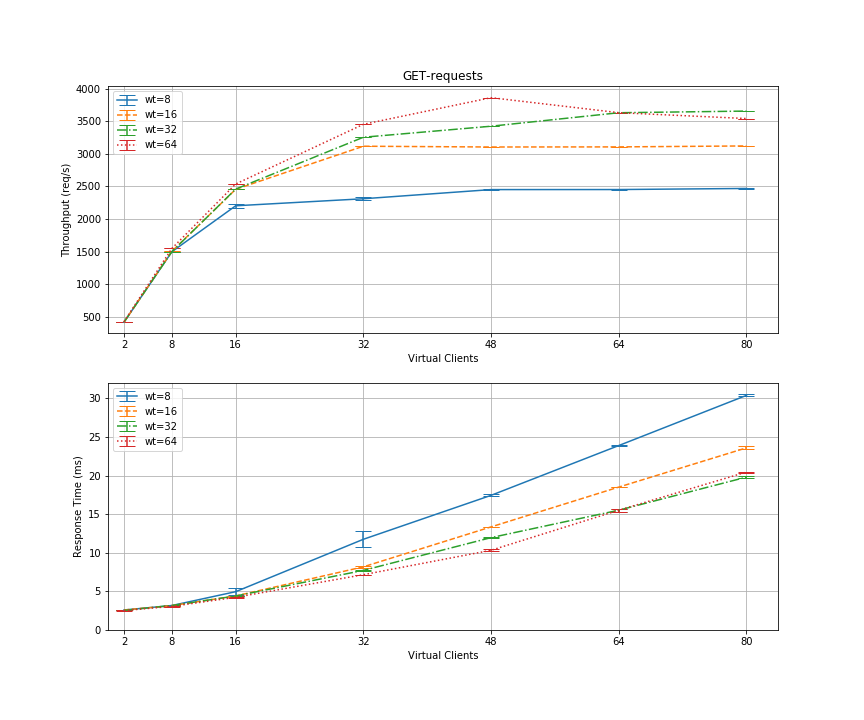
\includegraphics[width=.9\textwidth]{31/31_get_requests}
\caption{Experiment 3.1: Measured throughput and response time for a workload of only read requests. The middleware with 64 worker threads has the highest throughput and lowest response time. However, when the middleware with 64 workers goes into over-saturation phase, the throughput of the 32 thread system is still slowly rising. This suggests that while 64 threads may be optimal when it comes to maximum throughput, the 32 thread configuration may be more stable when the number of clients grows to above 48. This may be due to the added overhead of maintaining more threads.}
\label{fig:31_get}
\end{figure}

\begin{figure}
\centering
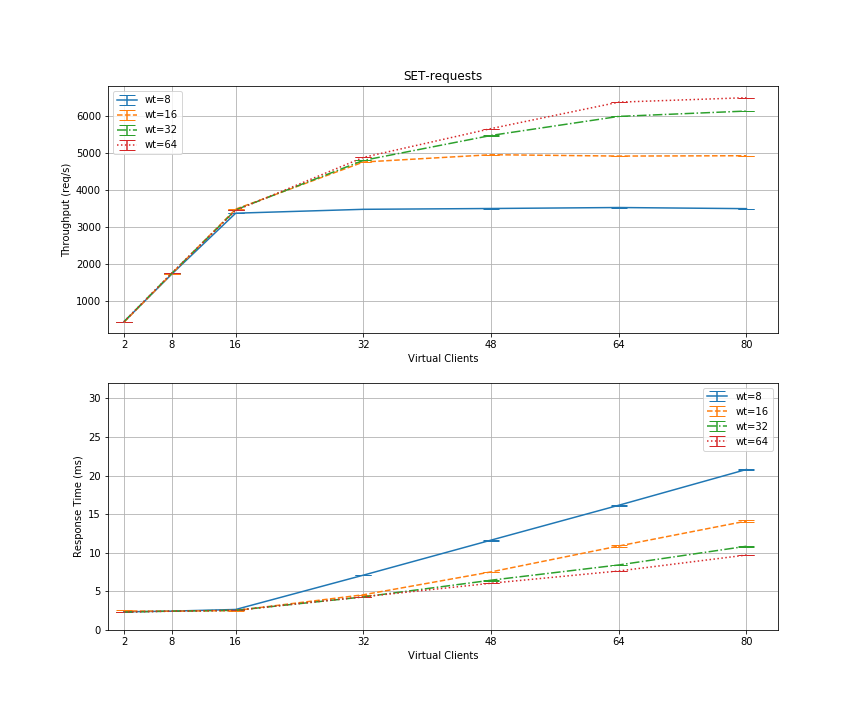
\includegraphics[width=.9\textwidth]{31/31_set_requests}
\caption{Experiment 3.1: Measured throughput and response time for a workload of only write requests. Similar to the result in the read-request experiments, the system with 64 threads has the highest throughput. However, unlike the write request case, the 64 thread middleware remains stable up until 80 clients, where our measurements end.}
\label{fig:31_set}
\end{figure}

\begin{figure}[t]
\centering
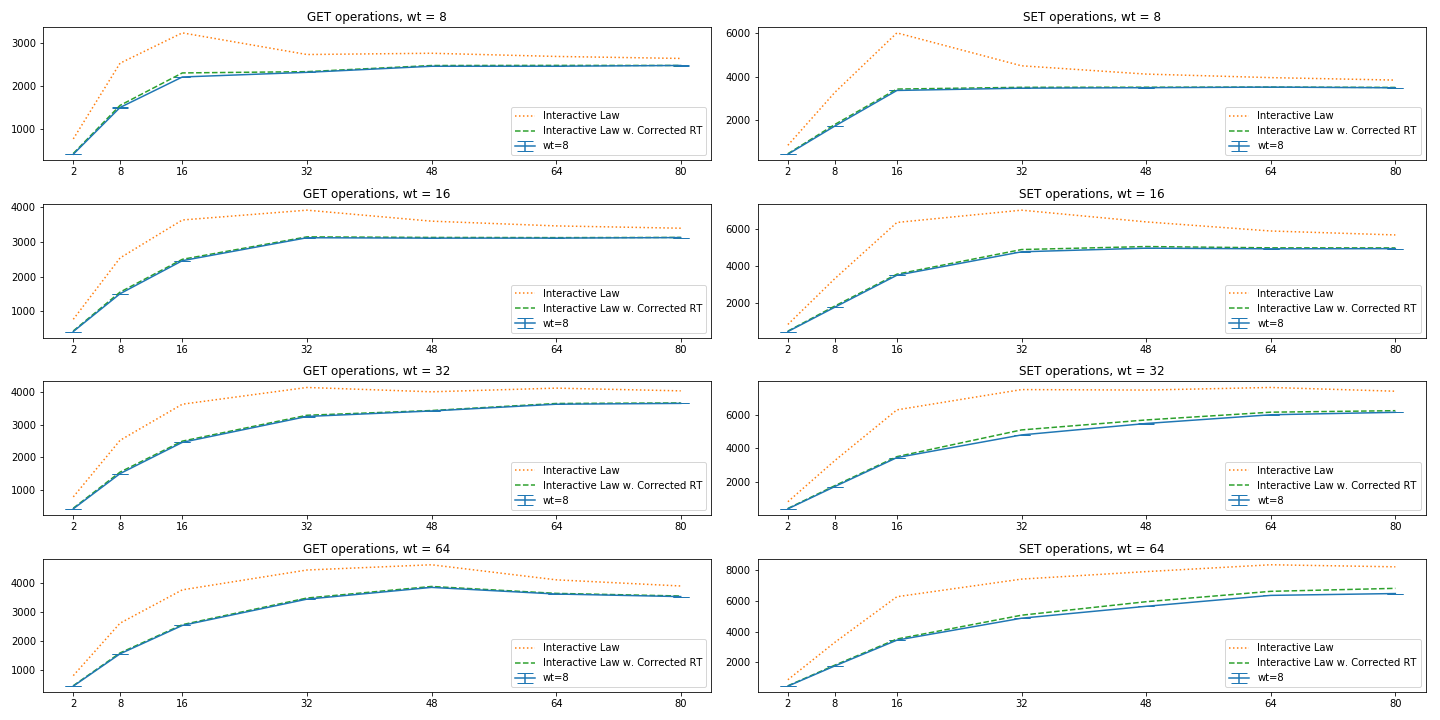
\includegraphics[width=1\textwidth]{31/31_interactive_law}
\caption{Experiment 3.1: A comparison of each of the experiments throughput and the throughput given by the interactive law. Using the response time measurements from the middleware to calculate the interactive law throughput, the measurements are far off. However, when the latency between the client and middleware are added to the response time measurements the measurements are very close to the interactive law predicted throughput.}
\label{fig:31_interactive_law}
\end{figure}

Unsurprisingly, the addition of the middleware to the system does not provide a benefit in the case of a single client and a single server. In this simple set-up the parsing of messages and extra latency incurred in the middleware slows the system down while no load-balancing or sharding of multi-gets is performed to increase the throughput (since it is not possible in this case).

\subsubsection{Interactive Law}
At first, the throughput and response time measurements from the middleware seem to not follow the interactive law, showing a lower throughput than what the interactive law predicts. This is due to the fact that the middleware response time measurements do not account for the latency between clients and the middleware. 

By comparing the response time measurements from the middleware and memtier\_benchmark, a constant difference of about 2ms was observed due to this latency. When a constant of 2ms is added to the measured response times in the middleware, the measured throughput and the interactive law prediction match quite well. The measured throughput, the predicted throughput according to response time measurements in the middleware and the predicted throughput according to the response time with this correction can all be observed in figure \ref{fig:31_interactive_law}.

\subsubsection{Bottleneck Analysis}
Using our measurements of response time, throughput and service time, we can calculate the utilization of the server and the middleware. The utilization of device $i$ is $U_i = X_i \cdot S_i$ where $X_i$ and $S_i$ are the throughput and service time of the device, respectively.

In our simple system $X_{middleware} = X_{server} = \mathrm{\textit{Total\ Throughput}}$ as measured on the middleware. For the service time of the middleware, we use $S_{middleware} = (RT-QT-ST)/WT$ where $RT$ is the measured response time in the middleware, $QT$ is the measured waiting time in the queue in the middleware and $ST$ is the middleware measured service time of the server. $WT$ is the number of worker threads in the middleware.

$RT$ is measured from when a request is put into the request queue until a response has been sent to the client. $QT$ is measured from when a request is put into the request queue, until it is removed from the queue. $ST$ is measured from when a request is sent to the server from the middleware until all servers have responded to the middleware.

For the service time of the server, $S_{server}$, we use minimum measured service times for each request type in experiments 3.1 and 3.2. They are $S_{server}^{get} = 0.122 ms$ and $S_{server}^{set} = 0.113 ms$.

Plugging these values into the equation: $U_i = X_i \cdot S_i$ we get the following device utilizations for the maximum throughput configurations:

\begin{center}
	{Utilization of devices\\}
	\begin{tabular}{|l|p{3cm}|p{3cm}|}
		\hline        & Server  [\%]                 & Middleware [\%]                             \\ 
		\hline GETS,  $wt=64$, $VC=24$     &    47       &       56         \\ 
		\hline SETS,  $wt=64$, $VC=40$     &    74       &       92        \\ 
		\hline 
	\end{tabular}
\end{center}

We see that for both read-only and write-only requests, the bottleneck of the system is the middleware. While the middleware is the bottleneck, it is interesting to see that the throughput of read-only requests with a single middleware is higher than in experiment 2.1, where the client was connected directly to the server (3862 req/s vs. 3650). This is likely to be due to variance or network effects, since it is hard to imagine how the middleware could increase the throughput between the client and server, especially since it is the bottleneck here.

In the case of writes, the throughput has gone quite a bit down from the results of experiment 2.1. Using this set up, we achieve a maximum of 6567 req/s compared to 7616 req/s in the baseline of experiment 2.1. This is not surprising considering that the middleware is at 92\% utilization.

Also note that the difference in utilization between devices is quite high in the case of write operations but lower in the case of read operations. This difference between request types can be explained by the overhead of the middleware and the added look up time for read requests on the server. In the case of read requests, the server needs to look up the value. The added service time due to look up causes the added overhead of the middleware to be of little consequence to the throughput. In the case of write requests, no look up is necessary on the server. The reduced service time on the server causes the middleware overhead to dominate and increasing the severity of the bottleneck of the system. 

The utilization of the client was not calculated. Since the throughput of this set up is much lower than the maximum measured in part 2.2 where the limits of the client are measured, we can conclude that the client is not a bottleneck here and its utilization does not need to be calculated.

\pagebreak
\subsection{Two Middlewares}
We now experiment with a set-up of one load generator VM with two single-thread (CT=1) instances of memtier, two middleware VMs and one memcached server. We explore how the behaviour of the system changes with the addition of another middleware.

\begin{figure}
\centering
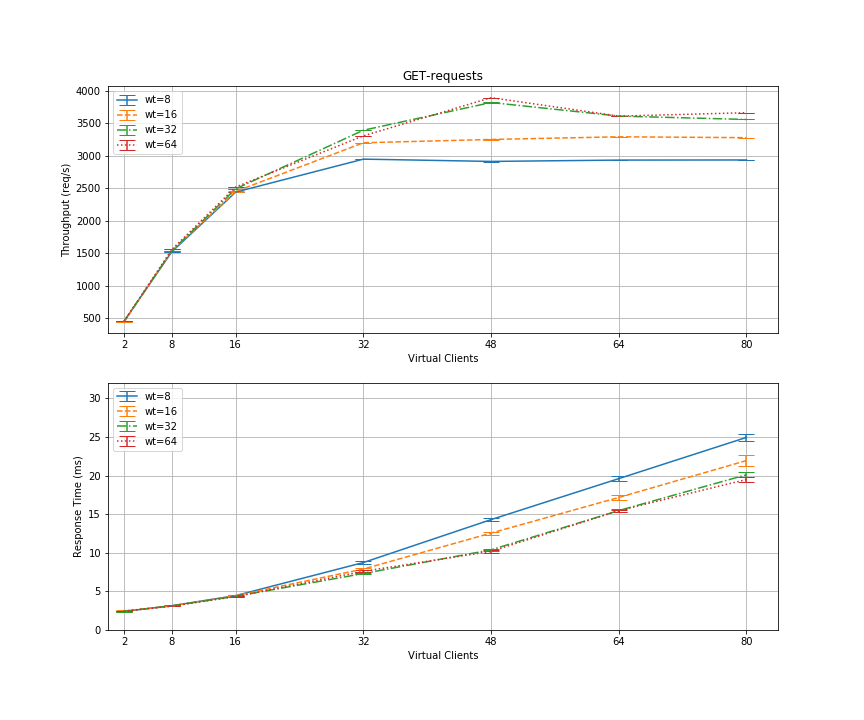
\includegraphics[width=.9\textwidth]{32/32_get_requests}
\caption{Experiment 3.2: Measured throughput and response time for a workload of only read requests. The middleware with 64 worker threads has the highest throughput and lowest response time while the 32 thread system come very close. A maximum throughput of 3894 req/s is measured.}
\label{fig:32_get}
\end{figure}

\begin{figure}
\centering
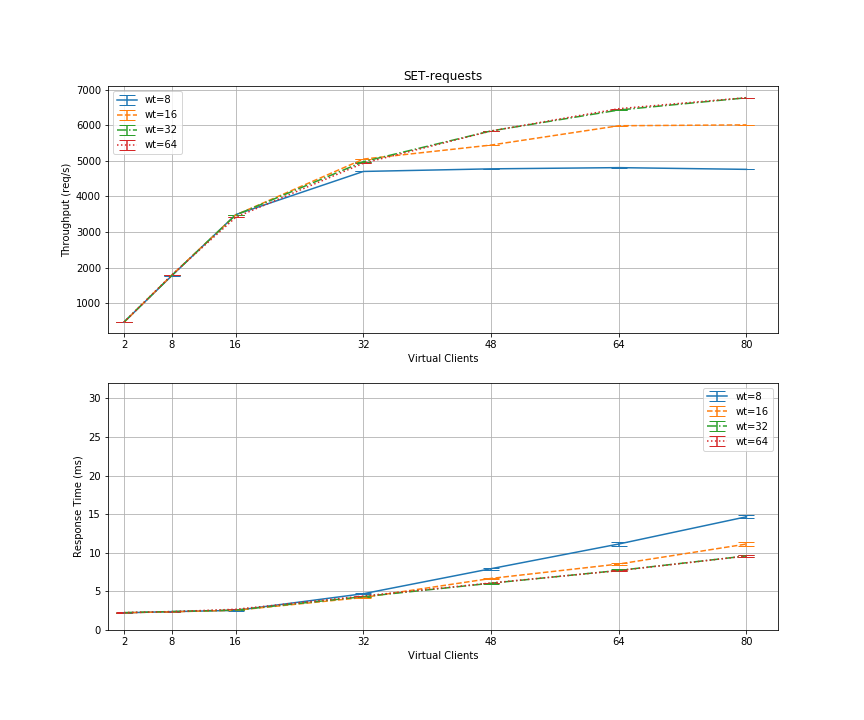
\includegraphics[width=.9\textwidth]{32/32_set_requests}
\caption{Experiment 3.2: Measured throughput and response time for a workload of only write requests. Similar to the result in the read-request experiments, the system with 64 threads has the highest throughput. Similar to the case of the read-only workload, the 32 thread configuration behaves almost exactly like the 32 thread configuration. A maximum throughput of 6774 req/s is measured.}
\label{fig:32_set}
\end{figure}

\begin{figure}[t]
\centering
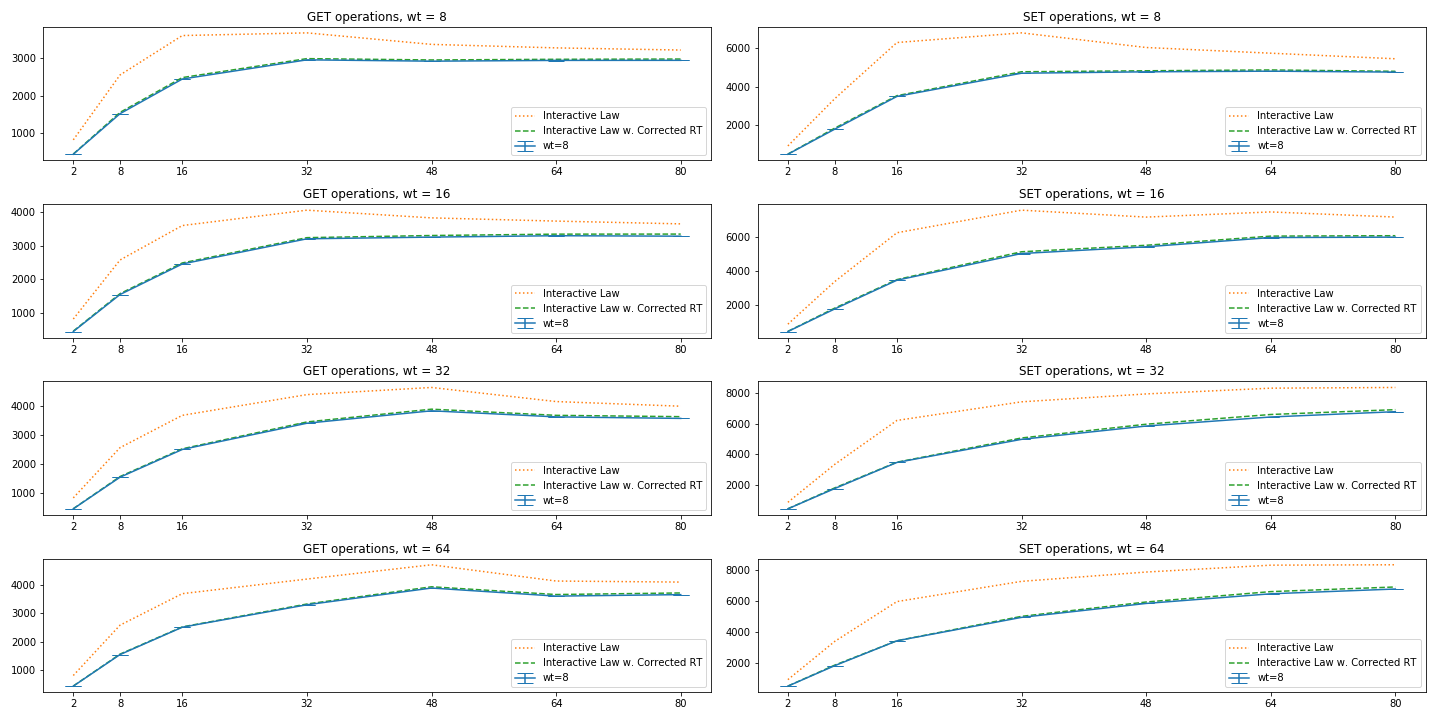
\includegraphics[width=1\textwidth]{32/32_interactive_law}
\caption{Experiment 3.2: A comparison of each of the experiments throughput and the throughput given by the interactive law. Using the response time measurements from the middleware to calculate the interactive law throughput, the measurements are far off. However, when the latency between the client and middleware are added to the response time measurements the measurements are very close to the interactive law predicted throughput.}
\label{fig:32_interactive_law}
\end{figure}

\pagebreak

\subsubsection{Bottleneck Analysis}
We calculate the utilization of the server and middlewares as before, however in this case we use the throughput measured through each middleware rather than the total throughput. The throughput for the server remains the total throughput as all requests are served by a single server.

\begin{center}
	{Utilization of devices\\}
	\begin{tabular}{|l|p{3cm}|p{3cm}|}
		\hline        & Server  [\%]                 & Middleware [\%]                             \\ 
		\hline GETS,  $wt=64$, $VC=24$     &    48       &       29         \\ 
		\hline SETS,  $wt=64$, $VC=40$     &    77       &       53        \\ 
		\hline 
	\end{tabular}
\end{center}

In both cases, the bottleneck in the system is the server. Note that the utilization of the server is very similar to our earlier experiment with 1 middleware as we would expect since the throughput is also very similar. However, the utilization of the middleware is about half of what was observed in experiment 3.1. This is due to the requests being equally divided between the two middlewares, indicating that adding another instance of the middleware is a good way to reduce the load on the middleware.

\pagebreak
\subsection{Two Middlewares, Two Client VMs}
Since the bottleneck was not the middleware in the previous experiment, we run an extra experiment with the maximum throughput configuration ($wt=64$) but with two load generating VMs instead of one.

\begin{figure}
\centering
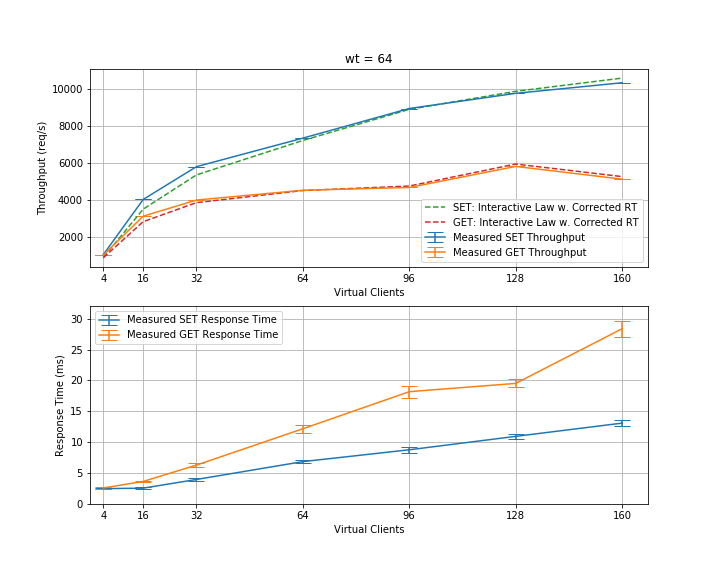
\includegraphics[width=.9\textwidth]{33/33_max_config}
\caption{Experiment 3.3: The results of adding another client to the system. The highest throughput for read requests was 5818 req/s and for write requests a throughput of 10349.8 was achieved. While these numbers are quite a bit higher than what was achieved in earlier experiments (2.1, 3.1 and 3.2), it is important to note that the virtual machines were stopped and restarted before doing experiment 3.3. Therefore, the performance metrics are NOT directly comparable to those achieved earlier.}
\label{fig:33_max_config}
\end{figure}

\subsubsection{Bottleneck Analysis}
\begin{center}
	{Utilization of devices\\}
	\begin{tabular}{|l|p{3cm}|p{3cm}|}
		\hline        & Server  [\%*]                 & Middleware [\%*]                             \\ 
		\hline GETS,  $wt=64$, $VC=32$     &    71       &       83         \\ 
		\hline SETS,  $wt=64$, $VC=40$     &    117      &       99        \\ 
		\hline 
	\end{tabular}
\end{center}
The server is the bottleneck for write requests while the middleware is the bottleneck for read requests.\\

*It is important to state here that all the virtual machines were stopped and then restarted before experiment 3.3 was run. This means that the network configuration of the machines is unlikely to be the same. This causes the calculation of utilization to be imprecise since network effects can dramatically affect the measured service times and throughput of both devices. This explains why a utilization above 100\% is calculated for the server. In light of this, the numerical value of the utilization should not be compared to earlier experiments or taken to be precise. However, they are still useful for comparing utilization of devices within this experiment.


\newpage

\subsection{Summary}

Based on the experiments above, we fill out the following table. For both of them we use the numbers from the single maximum throughput configuration to fill out all lines. Miss rate represents the percentage of GET requests that return no data. Time in the queue refers to the time spent in the queue between the net-thread and the worker threads.




\begin{center}
	{Maximum throughput for one middleware.}
	\begin{tabular}{|l|p{2cm}|p{2cm}|p{2.5cm}|p{1.5cm}|}
		\hline                                & Throughput & Response time [ms] & Average time in queue [ms] & Miss rate \\ 
		\hline Reads: Measured on middleware  &   3862     &     10.2      &   0.21             &  0.0029         \\ 
		\hline Reads: Measured on clients     &   3863     &     12.45     & n/a               &  0.093    \\ 
		\hline Writes: Measured on middleware &   6567     &     9.58      &   0.07            & n/a       \\ 
		\hline Writes: Measured on clients    &   6530     &     12.26      & n/a              & n/a       \\ 
		\hline 
	\end{tabular}
\end{center}

\begin{center}
	{Maximum throughput for two middlewares.}
	\begin{tabular}{|l|p{2cm}|p{2cm}|p{2cm}|p{2cm}|}
		\hline                                & Throughput & Response time [ms] & Average time in queue [ms] & Miss rate \\ 
		\hline Reads: Measured on middleware  &    3894    &     9.3       &   0.002               &  0.0026   \\ 
		\hline Reads: Measured on clients     &    3903    &     12.32     & n/a                   &  0.084     \\ 
		\hline Writes: Measured on middleware &    6774    &     8.95      &   0.002               & n/a       \\ 
		\hline Writes: Measured on clients    &    6782    &     11.8      & n/a                   & n/a       \\ 
		\hline 
	\end{tabular}
\end{center}

In experiment 3.1 we saw that the middleware handled well a read-only workload from a single client. The throughput was comparable to the baseline established in the baseline without the middleware (experiment 2.1) and utilization of the middleware was only around 56\%, saturating the server. During a write-only load, the middleware became the bottleneck of the system, only allowing for 6500 req/s while the baseline in 2.1 had a throughput of 7600 req/s. This is due to read operations being slower than write operations on the server. In this way the middleware could handle the maximum possible read-throughput of the server but not the maximum possible write-throughput.

To investigate this issue further, we add another middleware to experiment 3.2. Now using two middlewares, the system manages to improve slightly on both read- and write-only workloads, however still not reaching the baseline established in experiment 2.1 for write-only workloads. This is to be expected since the additional networking time required to send the request first to the middleware and then to the server is bound to slow the system as whole, compared to sending the request directly from client to server. While throughput did not rise much when adding a second middleware, the utilization of the middlewares fell to about half of their former values due to requests being equally divided between middlewares. This suggests that even if adding middlewares does not significantly increase throughput for a single client VM, it may be an effective way to scale for multiple client VMs.

Exploring how the two middlewares scale with multiple client VMs, we experiment with two client VMs in experiment 3.3. In this case, the throughput rises significantly for both write- and read-only workloads reaching: $X_{get} = 5818$ req/s and $X_{set} = 10350$ req/s. This is supporting evidence for our suggestion that multiple middlewares may scale very effectively when more client are added. Although these values are high, one should be wary of directly comparing them to the results of experiment 3.1 and 3.2 since the VMs were stopped and started between experiments 3.2 and 3.3.

In both experiments 3.1 and 3.2 the throughput of the 32-thread and 64-thread middlewares was very similar and close to the maximum achived. This suggests that the optimal number of threads should be close to one of these values or somewhere in between. While increasing the thread count helps by parallelizing handling of the requests, the overhead of maintaining many threads in a system which only has a limited number of cores leads to diminishing returns and likely even slow down when the thread count is set too high, although this was not observed for our choices of threads.

Finally, it is worth noting that the measured miss rate of the middleware is far lower than the miss rate measured in the client. Searching the middleware source code for bugs did not lead to further insight into this problem nor manage to fix it. Proposed are two possible explanations for this:

1. This is due to an elusive bug in the middleware that was not found.

2. When the experiments were run, the servers were populated once before running the experiments with expiration time of 9999 seconds or 2.8 hours. It happens that both experiments 3.1 and 3.2 took around 3 hours to run and the maximum throughput configuration was in both cases one of the last to be tested. This means that while these configurations were running, many of the data entries would expire at the same time causing get-misses. Since so many data entries expire at the same time the get miss ratio is highly dependant on between which times the ratio is calculated. Since the client measurements are run for roughly 15 seconds longer than the measurements of the middleware, many keys may have expired in that time period, causing the client to measure a much higher miss ratio than the middleware.


\newpage

\section{Throughput for Writes (90 pts)}

\subsection{Full System}

\begin{figure}
\centering

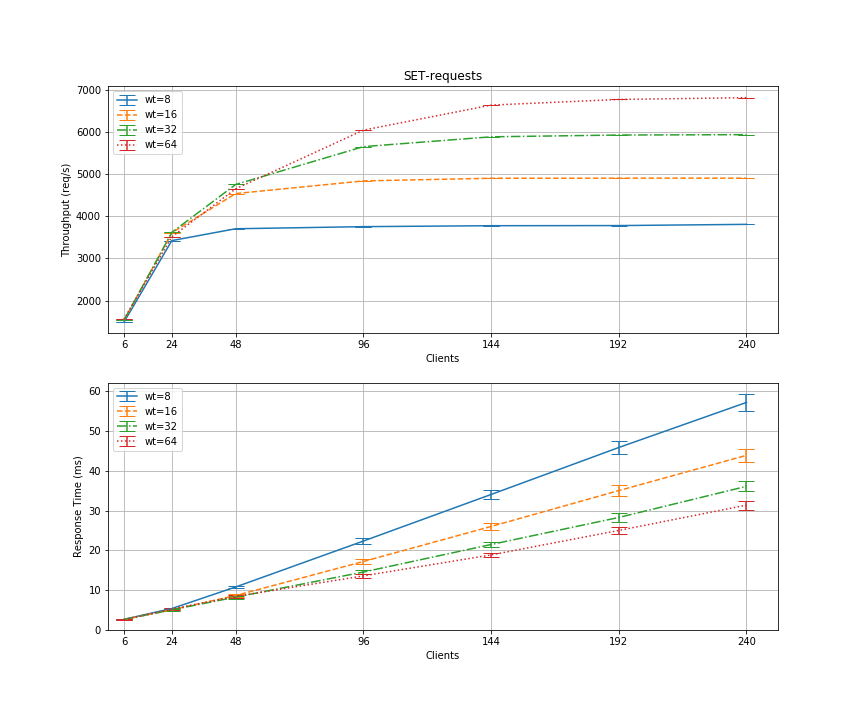
\includegraphics[width=1\textwidth]{41/41_set_requests}
\caption{Experiment 4.1: Throughput for write-only workloads on the full system. As seen in the baselines before, the highest throughput is achieved with 64 worker threads, achieving a throughput of 6814 req/s.}
\label{fig:41_set}
\end{figure}


We run an experiment with the full system and a Write-only workload. In this experiment, we connect three load generating client VMs to two middlewares and three memcached servers. We measure how throughput and response time depend on the number of clients for the following numbers of worker threads in the middleware: $WT = \{8, 16, 32, 64 \}$.

 \begin{figure}
\centering
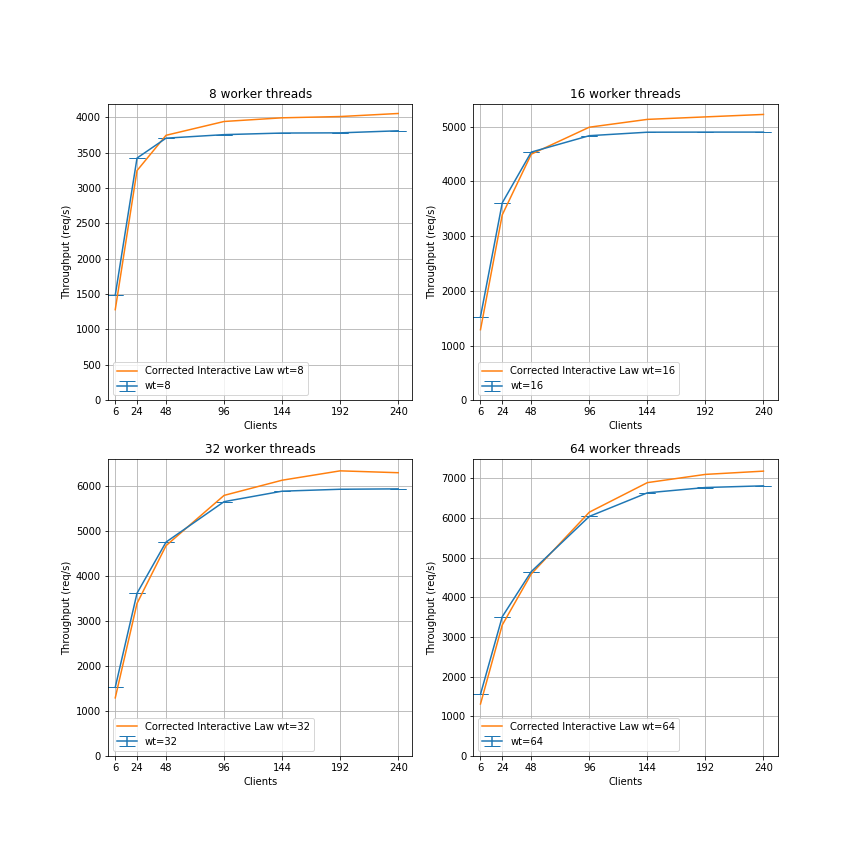
\includegraphics[width=1\textwidth]{41/41_il}
\caption{Experiment 4.1: Measured throughput for write-only workloads on the full system for all choices of worker threads. As can be seen in the table above, the middleware measured throughput is around 10\% lower than the throughput predicted by the interactive law. However, when comparing the response time measured in the middleware and in the clients difference of around 3 ms can be seen due to network effects. The interactive law plotted in these graphs have been calculated by adding 3 ms to all response times. This makes the interactive law fit better to the measured throughput. }
\label{fig:41_il}
\end{figure}


\subsection{Analysis}

\begin{center}
	{Maximum throughput for the full system}
	\begin{tabular}{|l|p{1.5cm}|p{1.5cm}|p{1.5cm}|p{1.5cm}|}
		\hline                                            & WT=8 & WT=16 & WT=32 & WT=64 \\ 
		\hline Throughput (Middleware)                    & 3807.2 & 4903.1 & 5934.7 & 6813.4 \\ 
		\hline Throughput (Derived from MW response time) & 4193.3 & 5464.1 & 6643.0 & 7641.5 \\ 
		\hline Throughput (Client)                        & 4090.0 & 5780.7 & 6353.3 & 7225.3 \\ 
		\hline Average time in queue [ms]                 & 19.258 & 8.545   & 3.476 & 1.026    \\ 
		\hline Average length of queue                    & 104   & 94    & 74    & 40    \\ 
		\hline Average time waiting for memcached [ms]    & 1.398 & 1.358 & 1.340 & 1.349  \\ 
		\hline 
	\end{tabular}
\end{center}

Note that there is around 10\% difference in throughput measured by middleware and throughput measured from client. This is due to the client measuring middleware during warm-up and cool-down phases. During warm-up there is no prior load on the middlewares or servers causing the first requests to be answered much quicker. As can be seen in the table, the queue wait time is significant in this case. This wait time is bypassed or lessened for the first few requests which are then measured by the client but not the middleware. As for the derived throughput from response time, it is higher than measured due to the latency between client and middleware. This latency is not measured in the response time of the middleware which causes the prediction to be too high. Adding 2ms to the response time to counterweigh this problem causes the predicted throughput and measured throughput to be more similar. See figure \ref{fig:41_il}.

From figure \ref{fig:41_set} we see that the system saturates at different points depending on the number of worker threads. For $WT=8$ the system is already saturated at 48 clients. For $WT=16$ the system saturates at 96 clients. For $WT=32$ the system saturates at 144 clients and for $WT=64$ at 192 clients.

Using our measurements of the system we analyze the utilization of the system components, $U_i = X_i \cdot S_i$. Here $X_i$ is the throughput through device $i$ and $S_i$ is the service time for a request in device $i$. We calculate server utilization using the total throughput since all SET requests must be sent to all servers and with the previously established service time for SET requests (see chapter 2.1). We calculate middleware utilization with $S_{middleware} = \frac{1}{Max\_throughput}$ where $Max\_throughput$ is is the highest throughput measured for the given configuration over the time windows measured in the middleware. 

\begin{center}
	{Device Utilization\\}
	\begin{tabular}{|l|p{3cm}|p{3cm}|}
		\hline              & Servers & Middlewares \\ 
		\hline WT=8         & 	43\%	 & 90\%	 \\ 
		\hline WT=16		 & 	55\%	 & 88\%	 \\ 
		\hline WT=32 		 & 	67\%	 & 90\%	 \\ 
		\hline WT=64        & 	77\%	 & 89\%   \\
		\hline 
	\end{tabular}
\end{center}

For all choices of $WT$, the middleware is the bottleneck. As $WT$ is increased, so does the throughput of the system. While throughput is increased, the utilization of the middleware remains around 90\% but the utilization grows significantly from 43\% to 77\%. This indicates that while the middleware is in all cases the bottleneck, the bottleneck effect is reduced for higher choices of the number of worker threads. As $WT$ grows, the servers become more utilized due to the increased throughput (almost doubling from 3807 req/s for $WT=8$ to 6813 req/s for $WT=64$) \\

When these results are compared with the statistcs in table \ref{table:2k}, it may at first seem like utilization of the middleware should be reduced for higher worker counts since both average queue time and average length of the queue are significantly reduced. However, upon closer inspection one sees that the reduction in the length of the queue is very close to the added number of threads. This suggests that for higher worker thread counts, instead of spending most of the time on the queue the requests spend more time in the worker threads.\\

It would be possible speed up the system by responding to the client when at least one server has responded instead of waiting for all servers to respond in the case of set requests. When the first server responds the set request will have been sent to all servers. Assuming that servers handle requests sequentially, this approach should not lead to new inconsistencies between servers and speed up the system. If this was implemented, it would be wise to have the worker thread wait for all servers to respond to ensure that the request has been successfully stored on all servers. If they are not stored, the middleware would need to handle that (e.g. by re-sending the request).

\newpage

\section{Gets and Multi-gets (90 pts)}

For this set of experiments we use three load generating machines, two middlewares and three memcached servers. Each memtier instance has 2 virtual clients in total and the number of middleware worker threads is 64, the maximum throughput configuration for our system.

We run a workload consisting of mixed SETs, GETs and multi-GETs. This is achieved by passing the following parameters: "\texttt{--multi-key-get=mk --ratio 1:mk}" to Memtier\_Benchmark where $\texttt{mk}$ is the number of desired keys in each multi-GET request. In contradiction to the report-outline, this approach does not specify the maximum number of keys in multi-GET requests but rather the number of keys in every multi-GET request. The average number of keys in the multi-GET requests was measured in the middleware, confirming this.

Using these measurements we explore how the response time changes as a function of multi-GET sizes for both middleware with and without sharding. In both cases we run the experiments for $mk = \{ 1, 3, 6, 9 \}$ keys in each multi-GET.

\subsection{Sharded Case}

Figure \ref{fig:51_all_req} shows the results of the experiment for the middleware with sharded GET-requests.

\begin{figure}
\centering
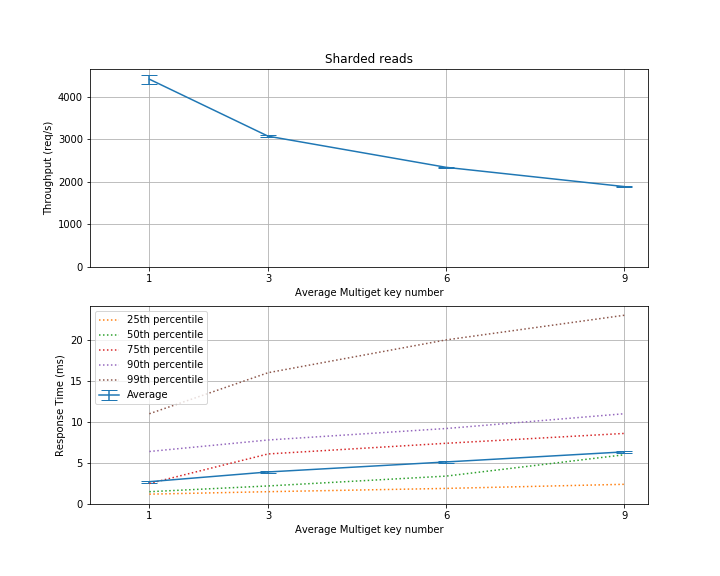
\includegraphics[width=.9\textwidth]{51/51_all_requests.png}
\caption{Experiment 5.1: Throughput and response times for multigets of various sizes in middleware with sharded GETs. Note how average response time rises linearly with key number. However the 99th percentile seems to rise sublinearly.}
\label{fig:51_all_req}
\end{figure}

\subsubsection{Analysis}
We perform bottleneck analysis on the system by calculating the utilization of each component. For the middleware we assume the service time to be $S_{middleware} = \frac{1}{3\cdot X_{max}}$ where $X_{max}$ is the maximum throughput observed in any client for each size of multigets. Since there are 3 clients connected to each middleware, we use three times this number to estimate the utilization of the middlewares. Then $U_{middleware} = X_{middleware} \cdot S_{middleware}$.\\

To estimate the utilization of the servers we use the average measured service time, $S_{server}$, for each size of multigets. This results in the following utilizations in table \ref{table:51_util}.

\begin{table}[h]
\centering
\caption{Utilization of components using sharded get requests.}
\label{table:51_util}
\begin{tabular}{l|cc}
       & \multicolumn{1}{l}{Middleware Utilization} & \multicolumn{1}{l}{Server Utilization} \\ \hline
1 Key  & 92.6\%                                     & 97.0\%                                 \\
3 Keys & 93.5\%                                     & 87.5\%                                 \\
6 Keys & 95.2\%                                     & 85.6\%                                 \\
9 Keys & 96.0\%                                     & 81.3\%                                
\end{tabular}
\end{table}

The utilization of the middleware is higher in all cases but in the case with single key GETs. There is no difference between "1 key multiGETs" and normal GETs. We see that the server is more utilized in that case, this should not come as a surprise. In earlier experiments, we have established that GET requests are handled slower on the server than SET operations while the difference between the requests types is negligible on the middleware.\\

For GET requests with more than one key, we notice that the middleware becomes the bottleneck. Parsing the request and dividing it into smaller request slows down the workers. In addition to this slow down, the worker needs to wait for the response from all servers thus being bound by the slowest server. This means that one server being slow or having unfortunate network conditions will slow down every GET request, rather than only those which were sent to it in the case of non-sharded GETs.

\subsection{Non-sharded Case}

Figure \ref{fig:52_all_req} shows the results of the experiment for the middleware with sharded GET-requests.

\begin{figure}
\centering
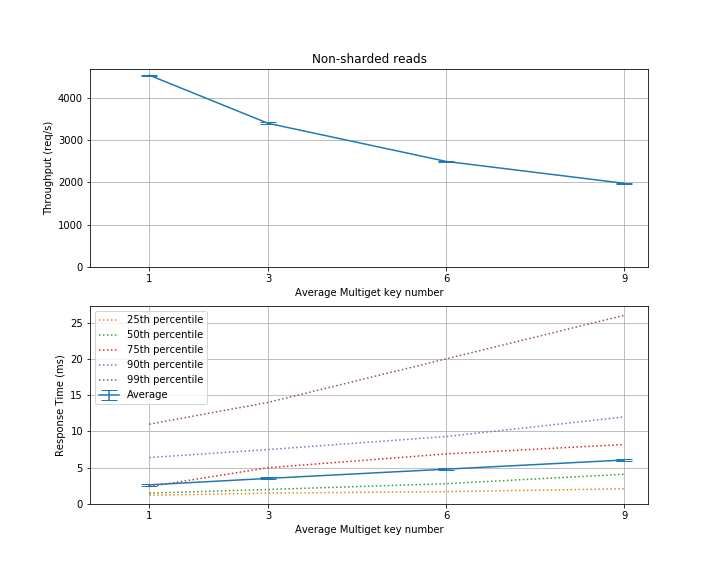
\includegraphics[width=.9\textwidth]{52/52_all_requests.png}
\caption{Experiment 5.2: Throughput and response times for multigets of various sizes in middleware with non-sharded GETs. Note how average response time rises linearly with key number. In this case, the 90th and 99th percentiles rise slightly super-linearly compared to slightly sub-linearly in the sharded case.}
\label{fig:52_all_req}
\end{figure}

\subsubsection{Analysis}
As before, we perform bottleneck analysis on the system by calculating the utilization of each component. Calculations are done in the same manner as before.

\begin{table}[h]
\centering
\caption{Utilization of components using non-sharded get requests.}
\label{table:52_util}
\begin{tabular}{l|cc}
       & \multicolumn{1}{l}{Middleware Utilization} & \multicolumn{1}{l}{Server Utilization} \\ \hline
1 Key  & 93.1\%                                     & 100.6\%                                \\
3 Keys & 94.7\%                                     & 96.8\%                                 \\
6 Keys & 95.3\%                                     & 95.3\%                                 \\
9 Keys & 97.2\%                                     & 94.3\%                                
\end{tabular}
\end{table}

In the case of non-sharded GET requests, the server tends to be more utilized for 1 and 3 keys per request. For 9 key requests, the middleware becomes more utilized, while utilization is virtually equal for 6 key requests. The bottleneck is thus the server in the first two cases but the middleware in the last case. 

\subsection{Histogram}

For the case with 6 keys inside the multi-get, display four histograms representing the sharded and non-sharded response time distribution, both as measured on the client, and inside the middleware. Choose the bucket size in the same way for all four, and such that there are at least 10 buckets on each of the graphs.

\begin{figure}[] 
  \begin{subfigure}[b]{0.5\linewidth}
    \centering
    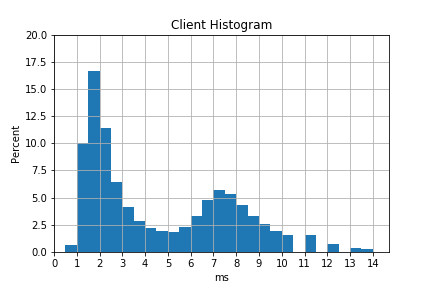
\includegraphics[width=1\linewidth]{51/51_client_histogram.png} 
    \caption{Sharded, Client measurements} 
    \label{fig7:a} 
    \vspace{4ex}
  \end{subfigure}%% 
  \begin{subfigure}[b]{0.5\linewidth}
    \centering
    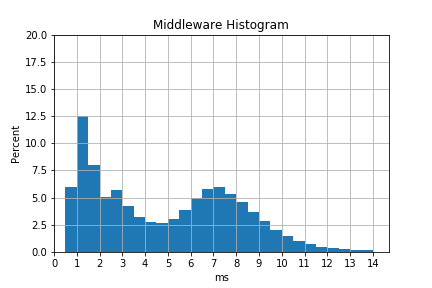
\includegraphics[width=1\linewidth]{51/51_mw_histogram.png} 
    \caption{Sharded, Middleware measurements} 
    \label{fig7:b} 
    \vspace{4ex}
  \end{subfigure}
  \begin{subfigure}[b]{0.5\linewidth}
    \centering
    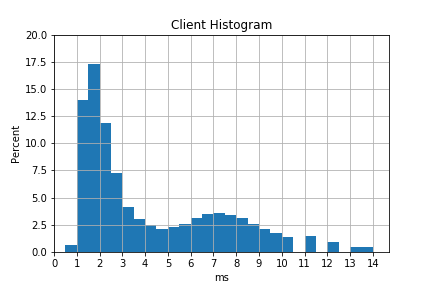
\includegraphics[width=1\linewidth]{52/52_client_histogram.png} 
    \caption{Non-Sharded, Client measurements} 
    \label{fig7:c} 
  \end{subfigure}%%
  \begin{subfigure}[b]{0.5\linewidth}
    \centering
    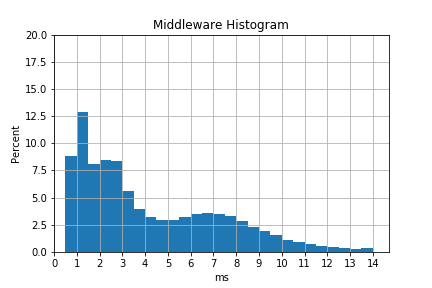
\includegraphics[width=1\linewidth]{52/52_mw_histogram.png} 
    \caption{Non-Sharded, Middleware measurements} 
    \label{fig7:d} 
  \end{subfigure} 
  \caption{Comparison of response times gathered from client and middleware and for the case of sharded and non-sharded GET requests for 6 keys per GET request. Interestingly, the clients tend to measure slightly shorter response times. In all histograms we see two "bumps", the first centered around 2 ms and the second centered around 7 ms. These two bumps represent the two different request types for the mixed workload. The first bump represents SET requests which all contain one key and one value. The second bump represents the multi-GET requests which contain 6 keys. We notice a more equal spread for non-sharded request, that is higher variance in response time. This is due to the requests only being sent to one server in the non-sharded case. In the case of sharded requests, the request is sent to all servers and the response time must include the time it takes the last server to respond. It is clear that this measurement has less variance than the response time of a single server.}
  \label{fig7} 
\end{figure}

\subsection{Summary}

Comparing the two configurations, sharded and non-sharded, we notice that the throughput is very similar but slightly lower for the case of sharded reads. Similarly, the response time is slightly increased for sharded reads. This holds for all multiGET lengths. At first glance this may seem to suggest that sharded reads are not an improvement but sharded reads may still have some merit.\\

When looking at the 90th and 99th percentiles of response times for each configuration we notice that these percentiles with non-sharded reads seem to grow slightly super-linearly while slightly sub-linearly for sharded reads. This suggests that while the sharded approach is in general slower, it may be an effective way of reducing the response time of the slowest of requests for larger key numbers. If the response time of the slowest requests are of more importance than the mean response time and if the server is expected to handle large multiGETs, sharded reading is likely to be a better approach.\\

The bottleneck analysis shows the middleware to be the bottleneck in most cases. However, the sharded approach reduces the utilization of the server by almost 10\% for GETs with 6 and 9 keys without reducing the throughput significantly. Depending on the costs of adding more middlewares versus servers, sharding may be a way to reduce the load on the more expensive machine.\\

While sharded GET requests show some promise, they have a serious flaw. Should one server become slow for some reason (e.g. malfunction or effects of the operating system) or be placed in an unfortunate place on the network, that server will then slow down every multiGET request sent to the system. Since the worker needs to wait for all servers to respond before responding to the client, this may lead to dramatic slow down or a complete crash of the system should the server go offline. 


\newpage

\section{2K Analysis (90 pts)}


For 3 client machines (with 64 total virtual clients per client VM) we measure the throughput and response time of our system in a 2k experiment with repetitions. All GET operations have a single key. We vary the following parameters:

\begin{itemize}
		
	\item Memcached servers: 2 and 3
	\item Middlewares: 1 and 2
	\item Worker threads per MW: 8 and 32
	      	      
\end{itemize}

We repeat the experiment for (a)~a write-only, (b)~a read-only, and (c)~a 50-50-read-write workload. We solve the resulting set of linear equations with the means of the throughput and response time as factors.


\begin{table}[h]
\centering
\caption{The effects of each parameter in the 2K analysis in percentages. The parameters are: $W=$ number of worker threads, $S=$ number of servers and $M=$ number of middlewares. The variation due to the number of worker threads is in all cases the largest by far. The variation due to the number of middlewares is the second highest in all cases but much lower than the variation due to the number of worker threads. Variation due to interaction of parameters is in most cases insignificant. However, in the case of response times of GETs, the interaction of worker threads and middlewares reaches 10\%.}
\label{table:2k}
\begin{tabular}{@{}l|lllllll@{}}
\toprule
                     & W     & S     & M     & W$\cdot$S & W$\cdot$M & S$\cdot$M & W$\cdot$S$\cdot$M \\ \midrule
Throughput: GET      & 49.07 & 19.70 & 25.68 & 1.36      & 3.40      & 0.77      & 0.02              \\
Throughput: SET      & 74.05 & 5.34  & 19.42 & 0.57      & 0.16      & 0.08      & 0.36              \\
Throughput: Mixed    & 70.76 & 1.37  & 27.45 & 0.01      & 0.97      & 0.03      & 0.42              \\ \midrule
Response Time: GET   & 50.36 & 14.69 & 23.51 & 0.40      & 10.70     & 0.11      & 0.24              \\
Response Time: SET   & 79.61 & 3.38  & 14.57 & 0.01      & 2.13      & 0.00      & 0.29              \\
Response Time: Mixed & 69.32 & 1.69  & 22.02 & 0.33      & 6.08      & 0.07      & 0.48              \\ \bottomrule
\end{tabular}
\end{table}

From table \ref{table:2k} we see that the number of worker threads is highly influential on the performance of our system. For both throughput and response time, for all types of requests, this parameter could be attributed to the largest part of the variation. This is especially prominent in the SET-workload. As we've seen in earlier experiments, the SET requests are handled quicker than GET requests on the server. Therefore, a speed up in the handling of SETs in the middleware is going to be highly influential on the performance of the whole system.

In all cases, the number of middlewares can be attributed to the second largest part of the variation. The effects of the server parameter is significant in the case of GETs due to their long service time on the server. The effects of parameter interaction are insignificant in all cases except Worker-Middleware interaction for the response time of GET requests. This interaction can be attributed 10.7\% of the variation of response time for GETs. 

In conclusion, the 2K analysis suggests that we should be especially interested in the number of worker threads in the middleware. For the testing range (8 and 32 worker threads) this parameter was by far of the most significance. The number of servers is not of high significane unless it is expected that the load will be mainly GET requests. For a SET workload or even a 50-50 mixed workload, this parameter is of relatively little effect for this testing range.

\section{Queuing Model (90 pts)}

Using the previous experimental results, we model our system with 3 different queuing models and compare to our measurements.

\subsection{M/M/1}

We build a queuing model based on Section 4 (write-only throughput) for each worker-thread configuration of the middleware, using one M/M/1 queue to model the entire system.\\

For the Arrival Rate, $\lambda$, we simply use the throughput of the system as a whole. Since the system is closed, the throughput should be equal to the arrival rate of requests into the system.

For the Service Rate, $\mu$, we use the maximum throughput measured over any time window in the middleware for the configuration.

We calculate the traffic intensity or utilization of our system as $\rho = \frac{\lambda}{\mu}$.\\

\begin{table}[h]
\centering
\caption{Arrival rate ($\lambda$), Service rate ($\mu$) and traffic intensity ($\rho$)}
\label{table:arrivalrate}
\begin{tabular}{l|llll}
          & 8 Workers & 16 Workers & 32 Workers & 64 Workers \\ \hline
$\lambda$ & 4222      & 5544       & 6602       & 7700       \\
$\mu$     & 3807    & 4903     & 5935     & 6813    \\
$\rho$    & 0.902     & 0.884      & 0.899      & 0.885     
\end{tabular}
\end{table}

Using these as our input parameters to the model, we calculate the following: Mean number of jobs in the system, mean number of jobs in the queue, mean response time and mean waiting time. The results of which can be seen in figure \ref{table:mm1}.

\begin{table}[h]
\centering
\caption{Calculated output variables of the model}
\label{table:mm1}
\begin{tabular}{l|llll}
                                  & 8 Workers & 16 Workers & 32 Workers & 64 Workers \\ \hline
Mean number of jobs in the system & 9.2       & 7.7        & 8.9        & 7.7        \\
Mean number of jobs in queue      & 8.3       & 6.8        & 8.0        & 6.8        \\
Mean Response Time {[}ms{]}       & 2.4       & 1.56       & 1.50       & 1.13       \\
Mean Queue Waiting Time {[}ms{]}        & 2.17      & 1.38       & 1.35       & 1.00      
\end{tabular}
\end{table}

Comparing these results with the measurements from chapter 4.1, we quickly see that the model does a bad job of approximating the system. By using the M/M/1 model, we are assuming that the system handles the requests in a sequential, non-parallel manner. Since the input parameters of the model are simply the maximum throughput achieved by all threads the model will approximate a single thread system with the same input as our multithreaded model but achieving the same throughput. It is obvious that this kind of modelling cannot be very accurate. It is interesting to see that the predicted values for queue waiting time are close to their measured values for 32 and 64 worker threads.

\subsection{M/M/m}

We now model the system with the M/M/m model with each middleware worker thread represented as one service. That is, $m$ is equal to the total number of worker threads in both middlewares: $m \in \{16, 32, 64, 128\}$.

\begin{table}[h]
\centering
\caption{Arrival rate ($\lambda$), Service rate ($\mu$) and traffic intensity ($\rho$)}
\label{table:mmminput}
\begin{tabular}{l|llll}
          & 8 Workers & 16 Workers & 32 Workers & 64 Workers \\ \hline
$\lambda$ & 4222      & 5544       & 6602       & 7700       \\
$m\mu$     & 3807    & 4903     & 5935     & 6813    \\
$\rho$    & 0.902     & 0.884      & 0.899      & 0.885     
\end{tabular}
\end{table}


\begin{table}[h]
\centering
\caption{Calculated output variables of the M/M/m model}
\label{table:mmmoutput}
\begin{tabular}{l|llll}
                                  & 8 Workers & 16 Workers & 32 Workers & 64 Workers \\ \hline
Mean number of jobs in the system & 20.67     & 31.95      & 61.73      & 114.54     \\
Mean number of jobs in queue      & 6.14      & 3.44       & 3.54       & 0.99       \\
Mean Response Time {[}ms{]}       & 5.43      & 6.51       & 10.40      & 16.8       \\
Mean Queue Waiting Time {[}ms{]}        & 1.61      & 0.70       & 0.60       & 0.14      
\end{tabular}
\end{table}

We calculate the output values seen in table \ref{table:mmmoutput}. Much like the M/M/1 model, the output values are not very close to the measured values. For 32 and 64 worker threads, the model outputs a reasonable number of jobs in the system although the number of jobs in the queue is much too low compared to our measurements. \\

Altough the M/M/m model is significantly more complex, it is still not able to approximate our system well. In using the M/M/m model we assume that all m services operate independently and the servers are not accounted for in the model but are rather a part of the m services which represent the workers. Both assumptions are bold. The workers are not independent since they operate on shared resources and the servers should be modelled as their own device rather than being a part of the workers.

\subsection{Network of Queues}

Based on Section 3, we build a network of queues which simulates your system. We implement the MVA algorithm as seen below. It has the following inputs $N=$ number of users, $Z=$ think time, $M=$ number of devices, $S=$ service times of devices, $V=$ visit ratio of devices.\\

For the simulation of the experiment in chapter 3.1, we create a model consisting of the following parts: The Network+NetHandler are modelled as one delay station with a service time of 2 ms. This is the average time it took requests to arrive from the client and be put into the queue in the middleware. We model the request queue as a fixed capacity service with zero service time. The workers are modelled as one delay station with the service time of the mean response time measured in experiment 3.1. The visit ratio of the worker is $1/wt$ where $wt$ is the number of worker threads in the configuration. Finally, the server is modelled as a fixed capacity service with service time 0.7 ms, the average measured service time of the middleware. Using these parameters we, plot the results of our model.

\begin{figure}
\centering
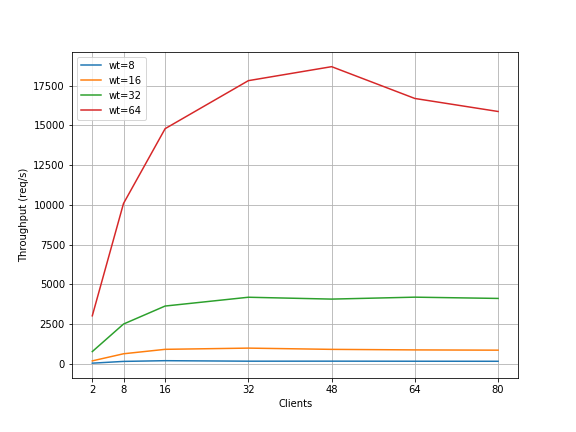
\includegraphics[width=.8\textwidth]{71/71_31get.png}
\caption{Throughput of the model of experiment 3.1 for GET requests.}
\label{fig:71_get}
\end{figure}

\begin{figure}
\centering
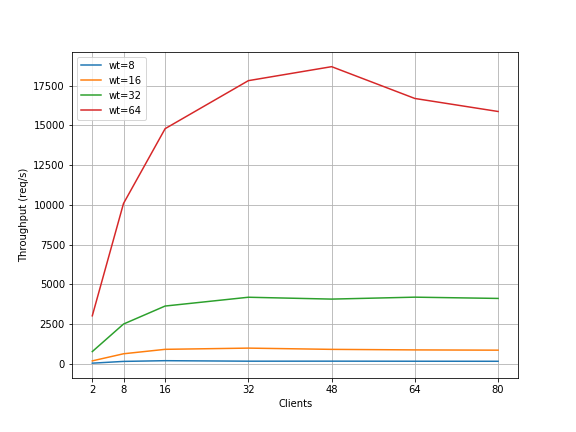
\includegraphics[width=.8\textwidth]{71/71_31set.png}
\caption{Throughput of the model of experiment 3.1 for SET requests.}
\label{fig:71_set}
\end{figure}

While the throughputs of both SET and GET workload are far from the measured values, we still see that the throughput curves look like those observed in chapter 3.1. In both cases the throughput of the model is much too high. This is due to the assumption that the worker threads operate in complete parallel and are not influence by each other. This assumption is made when the visit ratio of the worker service was set to $1/wt$ where $wt$ is the number of worker threads. A better approximation would like be possible, if the workers were modelled as a M/M/wt system. This, however, is not supported by the simple MVA algorithm. For GET requests, the worker was the bottleneck of the system for the maximum throughput configuration. For SET requests, the utilization of the NetHandler+Network service was at 58\% while the utilization of the middleware was at 47\%, with the other utilizations being far lower. This is not consistent with our results from chapter 3.1, where the utilization of the server was in all cases found to be the highest. Improvements on this model may be made by adjusting the input parameters of the model as well as using a more complex algorithm than the MVA, which support M/M/wt services.


\subsection{MVA algorithm implementation}
\begin{lstlisting}[language=Python]
def MVA(N,Z,M,S,V, device_type):
    # Inputs:
    # N = Number of users
    # Z = think time
    # M = Number of devices
    # S = Service time per visit to the ith device
    # V = Number of visits to the ith device

    # Device types, 0 = Fixed capacity, 1 = Delay center

    # Outputs:
    # X_sys System Throughput
    # Q[i] Avg. number of jobs at the ith device
    Q = np.zeros(M)
    # R[i] Response time of the ith device
    R = np.zeros(M)
    # R_sys System Response time
    # U[i] Utilization of ith device 
    U = np.zeros(M)
    for n in xrange(0,N):
        for i in xrange(0,M):
            if device_type[i] == 0:
                R[i] = S[i]*(1+Q[i])
            else:
                R[i] = S[i]

        R_sys = np.sum(np.multiply(R,V))
        X_sys = N/(Z+R_sys)

        for i in xrange(0,M):
            Q[i] = X_sys*V[i]*R[i]

    # Device throughputs
    X = np.multiply(X_sys,V)
    # Device utilizations
    U = np.multiply(X_sys, np.multiply(S,V))
    return X_sys, Q, R, R_sys, U, X


\end{lstlisting}
\end{document}
